
% Common Header for Artificial Intelligence class.
% Compile through etex to cache the header.
% Recipe: recompile header in VS Code

\documentclass[UTF8,12pt,a4paper]{ctexart}
\usepackage{amsmath,amscd,amsbsy,amssymb,latexsym,url,bm,amsthm}
\usepackage{epsfig,graphicx,subfigure}
\usepackage{enumitem,balance}
\usepackage{wrapfig}
\usepackage{array,float,booktabs}
\usepackage{mathrsfs,euscript}
\usepackage[usenames]{xcolor}
\usepackage{hyperref}
\usepackage[vlined,ruled,linesnumbered]{algorithm2e}
\hypersetup{colorlinks=true,linkcolor=black, citecolor=blue}
\usepackage{geometry}
\geometry{top=3cm,bottom=2cm,left=2cm,right=2cm}
\linespread{1.0}
\graphicspath{{img/}}

\newtheorem{theorem}{定理}
\newtheorem{lemma}[theorem]{引理}
\newtheorem{proposition}[theorem]{命题}
\newtheorem{corollary}[theorem]{推论}
\theoremstyle{definition}\newtheorem{problem}{题目}
\theoremstyle{plain}\newtheorem*{solution}{Solution}
\newtheorem{definition}{定义}

\makeatletter
\def\@maketitle{
    \noindent\framebox[\linewidth]{\shortstack[c]{
    \Large{\textbf{\@title}}\vspace{1mm}\\
    人工智能 \quad CS410 \quad 2021年秋季}}
    \begin{center}
        \footnotesize{
            \color{blue} 
            姓名:\@author \quad 
            学号:518070910095 \quad 
            日期:\@date
        }
    \end{center}
    \smallskip
}
\renewenvironment{proof}[1][证明]{\par\pushQED{\qed}\normalfont\topsep6\p@\@plus6\p@\relax\trivlist\item[\hskip\labelsep\bfseries#1\@addpunct{.}]\ignorespaces}{\popQED\endtrivlist\@endpefalse}
\renewenvironment{solution}[1][解] {\par\pushQED{\qed}\normalfont\topsep6\p@\@plus6\p@\relax\trivlist\item[\hskip\labelsep\bfseries#1\@addpunct{.}]\ignorespaces}{\popQED\endtrivlist\@endpefalse}
\makeatother

\usepackage{enumitem}
\setlist{nosep}
\setlist[enumerate]{label=(\arabic*)}

\usepackage{tikz}
\usepackage{pgfplots}
\pgfplotsset{compat=newest}
\usetikzlibrary{external}

\usepackage{gbt7714}


\usepackage{listings}
\definecolor{grey}{rgb}{0.8,0.8,0.8}
\definecolor{darkgreen}{rgb}{0,0.3,0}
\definecolor{darkblue}{rgb}{0,0,0.3}
\lstset{%
    columns=flexible,
    inputencoding=utf8,
    basicstyle=\small\ttfamily,
    numberstyle=\scriptsize\ttfamily\color{gray},
    showstringspaces=false,
    showspaces=false,%
    tabsize=4,
    numbers=left,
    framexleftmargin=8mm,
    xleftmargin=8mm,
    keepspaces=true,
    frame=lines,
    framerule=1pt,
    rulecolor=\color{green!50!black},
    backgroundcolor=\color{green!5},
    commentstyle=\color{gray}\itshape,
    stringstyle=\color{red!75},
    keywordstyle=\color{blue!80!black},
    lineskip=-1pt,
    breaklines,
    extendedchars=false
}
\providecommand{\code}[2][]{\lstinputlisting[caption=\href{./#2}{\ttfamily #2},#1]{#2}}
\providecommand{\codeseg}[4][]{\lstinputlisting[caption=\href{./#2}{\ttfamily #2},firstline=#3,firstnumber=#3,lastline=#4,#1]{#2}}
\lstdefinestyle{commandshell}{
    language=bash,numbers=none,frame=single,frameround=fttt,basicstyle=\normalsize\ttfamily
}  % usage: \begin{lstlisting}[style=commandshell]

\usepackage{multicol}

\def\filelink#1{
    \href{./#1}{\ttfamily #1}
}

\author{李子龙}

\begin{document}
    \title{第一次作业}
    \maketitle
    \begin{problem}
        示例题目
    \end{problem}
    \begin{solution}
        示例解法
        \begin{definition}
            示例定义
        \end{definition}
        \begin{enumerate}
            \item 1
            \item 2
            \item 3
        \end{enumerate}
        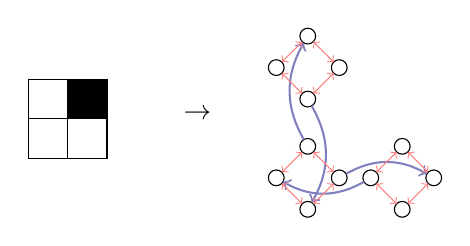
\begin{tikzpicture}
      \tikzstyle{bordered} = [draw,outer sep=0,inner sep=1,minimum size=0.5cm]
      \tikzstyle{state} = [draw,circle,outer sep=0,inner sep=1,minimum size=0.2cm]
      \tikzstyle{move}=[->,bend left,line width=0.75pt,blue!50!black!50]
      \tikzstyle{turn}=[<->,red!50]
	\node [bordered] at (-0.5,0) {};
\node [bordered,fill] at (0,0) {};
\node [bordered] at (-0.5,-0.5) {};
\node [bordered] at (0,-0.5) {};
\node [state] (v9) at (2.4,0.4) {};
\node [state] (v4) at (2.8,0.8) {};
\node [state] (v10) at (3.2,0.4) {};
\node [state] (v1) at (2.8,0) {};
\node [state] (v3) at (2.8,-0.6) {};
\node [state] (v8) at (2.4,-1) {};
\node [state] (v2) at (2.8,-1.4) {};
\node [state] (v5) at (3.2,-1) {};
\node [state] (v7) at (3.6,-1) {};
\node [state] (v11) at (4,-0.6) {};
\node [state] (v6) at (4.4,-1) {};
\node [state] (v12) at (4,-1.4) {};
\draw [move] (v1) edge (v2);
\draw [move] (v3) edge (v4);
\draw [move] (v5) edge (v6);
\draw [move] (v7) edge (v8);
\draw [turn] (v4) edge (v9);
\draw [turn] (v9) edge (v1);
\draw [turn] (v1) edge (v10);
\draw [turn] (v10) edge (v4);
\draw [turn] (v3) edge (v8);
\draw [turn] (v8) edge (v2);
\draw [turn] (v2) edge (v5);
\draw [turn] (v5) edge (v3);
\draw [turn] (v7) edge (v11);
\draw [turn] (v11) edge (v6);
\draw [turn] (v12) edge (v6);
\draw [turn] (v12) edge (v7);
\node at (1.4,-0.2) {$\rightarrow$};
\end{tikzpicture}
    \end{solution}
\end{document}